\section{Introduction}

This project has the aim of optimize a set of four queries from the \href{www.tpc.org/tpc\_documents\_current\_versions/pdf/tpch\_v3.0.1.pdf}{TPC benchmark H}
The database consists of eight tables: customer, lineitem,
nation, orders, part, partsupp, region, supplier. The relations between tables can be seen in the schema in figure \ref{fig:rel_schema}.

\begin{figure}[h!]
    \centering
    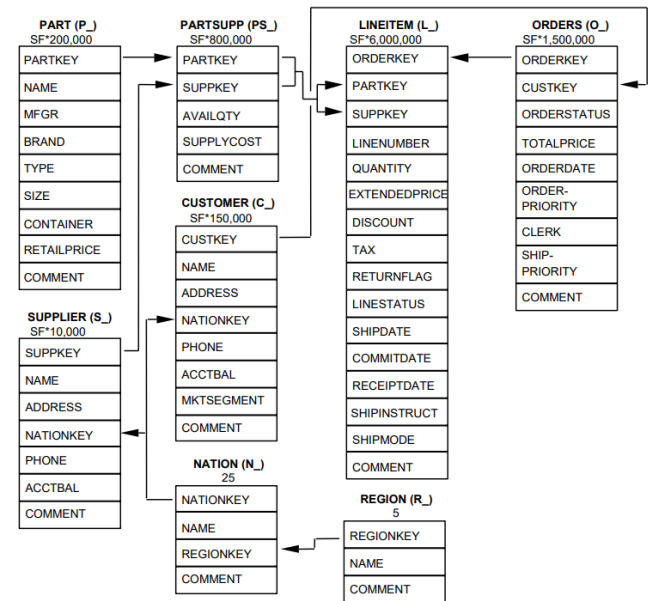
\includegraphics[scale=0.45]{images/rel_schema.png}
    \caption{Schema of the relaction between tables in the TPC-H benchmark}
    \label{fig:rel_schema}
\end{figure}

\subsection{Creation and population of the database}

The size of the database is scalable, and depends on a scale factor (SF), and we were given data generated from $SF=10$. Each table, from the documentation, has its own primary key and one or more foreign keys. Complete description of the table can be found \href{www.tpc.org/tpc\_documents\_current\_versions/pdf/tpch\_v3.0.1.pdf}{here}, while the complete SQL tables implementation and creation can be found \href{https://github.com/ValentinisAlessio/DM_Final_Project/blob/main/dbms.ipynb}{here}.

For the purpose of space economy, we opted for an initial "vanilla" creation of the tables, without any kind of keys: this choice is furthermore supported by the fact that we are dealing with a Data Warehousing context, so we expect the data to be already prepared and cleaned from duplicates.

After having populated the tables, we inserted all the keys reported in the documentation in order to work properly with the relations. However, always for the purpose of gaining some space, we decided not to implement the \textit{Primary key} to the Main table \texttt{lineitem}, as (for the same purposes described above,) we don't need to check for uniqueness constraints during the population of the Database, and for the sake of optimization, a simple index should help us to spare some pretty useful space.

In the table \ref{tab:table_dimensions}, we provide some information about the dimension of the various tables, in increasing order.

\begin{table}[h!]
\centering
\begin{tabular}{c|c|c|c}
\rowcolor{blue!50} Table & Number of rows & Dim without keys (MB) & Dim with keys (MB)\\
\rowcolor{gray!10} region & 5 & 0.01 & 0.02\\ 
\rowcolor{white} nation & 25 & 0.01 & 0.02\\ 
\rowcolor{gray!10} supplier & 100000 & 17.35  & 19.51 \\ 
\rowcolor{white} customer & 1500000& 290.17  & 322.32 \\ 
\rowcolor{gray!10} part & 2000000 & 320.14  & 363.00 \\ 
\rowcolor{white} partsupp & 8000000 & 1362.80  & 1535.12 \\
\rowcolor{gray!10} orders & 15000000 & 2038.97  & 2360.30 \\
\rowcolor{white} lineitem & 59986052 & 8787.95  & 10073.67 \\
\end{tabular}\\[0.5cm]
    \caption{General statistics}
    \label{tab:table_dimensions}
\end{table}

\subsection{Measurement techniques}

In order to assess the performance of the various queries, we used the 
\verb|EXPLAIN ANALYZE| feature of \textit{PostgreSQL} (per gli amici Postgress). It provided a complete summary of the execution plan of the queries, and provides also the execution time in milliseconds.
In order to have some significance on the result, we executed every query 5 times, and then we computed the mean and standard deviation of the measurements.

In order to keep track of the dimension of the database, we used the 
\verb|SELECT| \\
\verb|pg_database_size();| command, and convert the dimension in MB or GB.

\subsection{Hardware specifications}

All the test were conducted on a MacBook Air laptop with the following characteristics:
\begin{itemize}
    \item CPU: Chip Apple M2, 8 core (4 performance cores and 4 efficiency cores);
    \item RAM: 8GB;
    \item SSD: SATA 256GB;
    \item GPU: built-in 10 cores GPU;
    \item OS: macOS Sonoma 14.2.1.
\end{itemize}